\chapter{Introducere}
\label{chapter:intro}

\par Proiectul de față este un plugin care vine în ajutorul developerilor și designerilor de aplicații user experience.
\par În capitolul acesta, se va realiza o scurtă descriere a proiectului, motivația și obiectivele aplicatiei, iar  în urmatoarele secțiuni se va detalia arhitectura și modul de implementare al acesteia.

\section{Descrierea proiectului}
\label{sec:proj}
\par Lucrarea are ca temă realizarea managementului elementelor vizuale printr-o translatare între diferite reprezentări.  
\par O primă reprezentare este una logică, definită prin Xcode Interface Builder. Cea de-a doua reprezentare este definită prin produsul software Adobe Eperience Design (XD). 
Pentru implementarea acestui proiect s-a luat în considerare structura internă a fișierelor corespunzătoare celor 2 aplicații.

\begin{figure}[!htbp]
\centering
\begin{tikzpicture}[node distance = 4cm, auto]
\node (xd) at (0, 0) {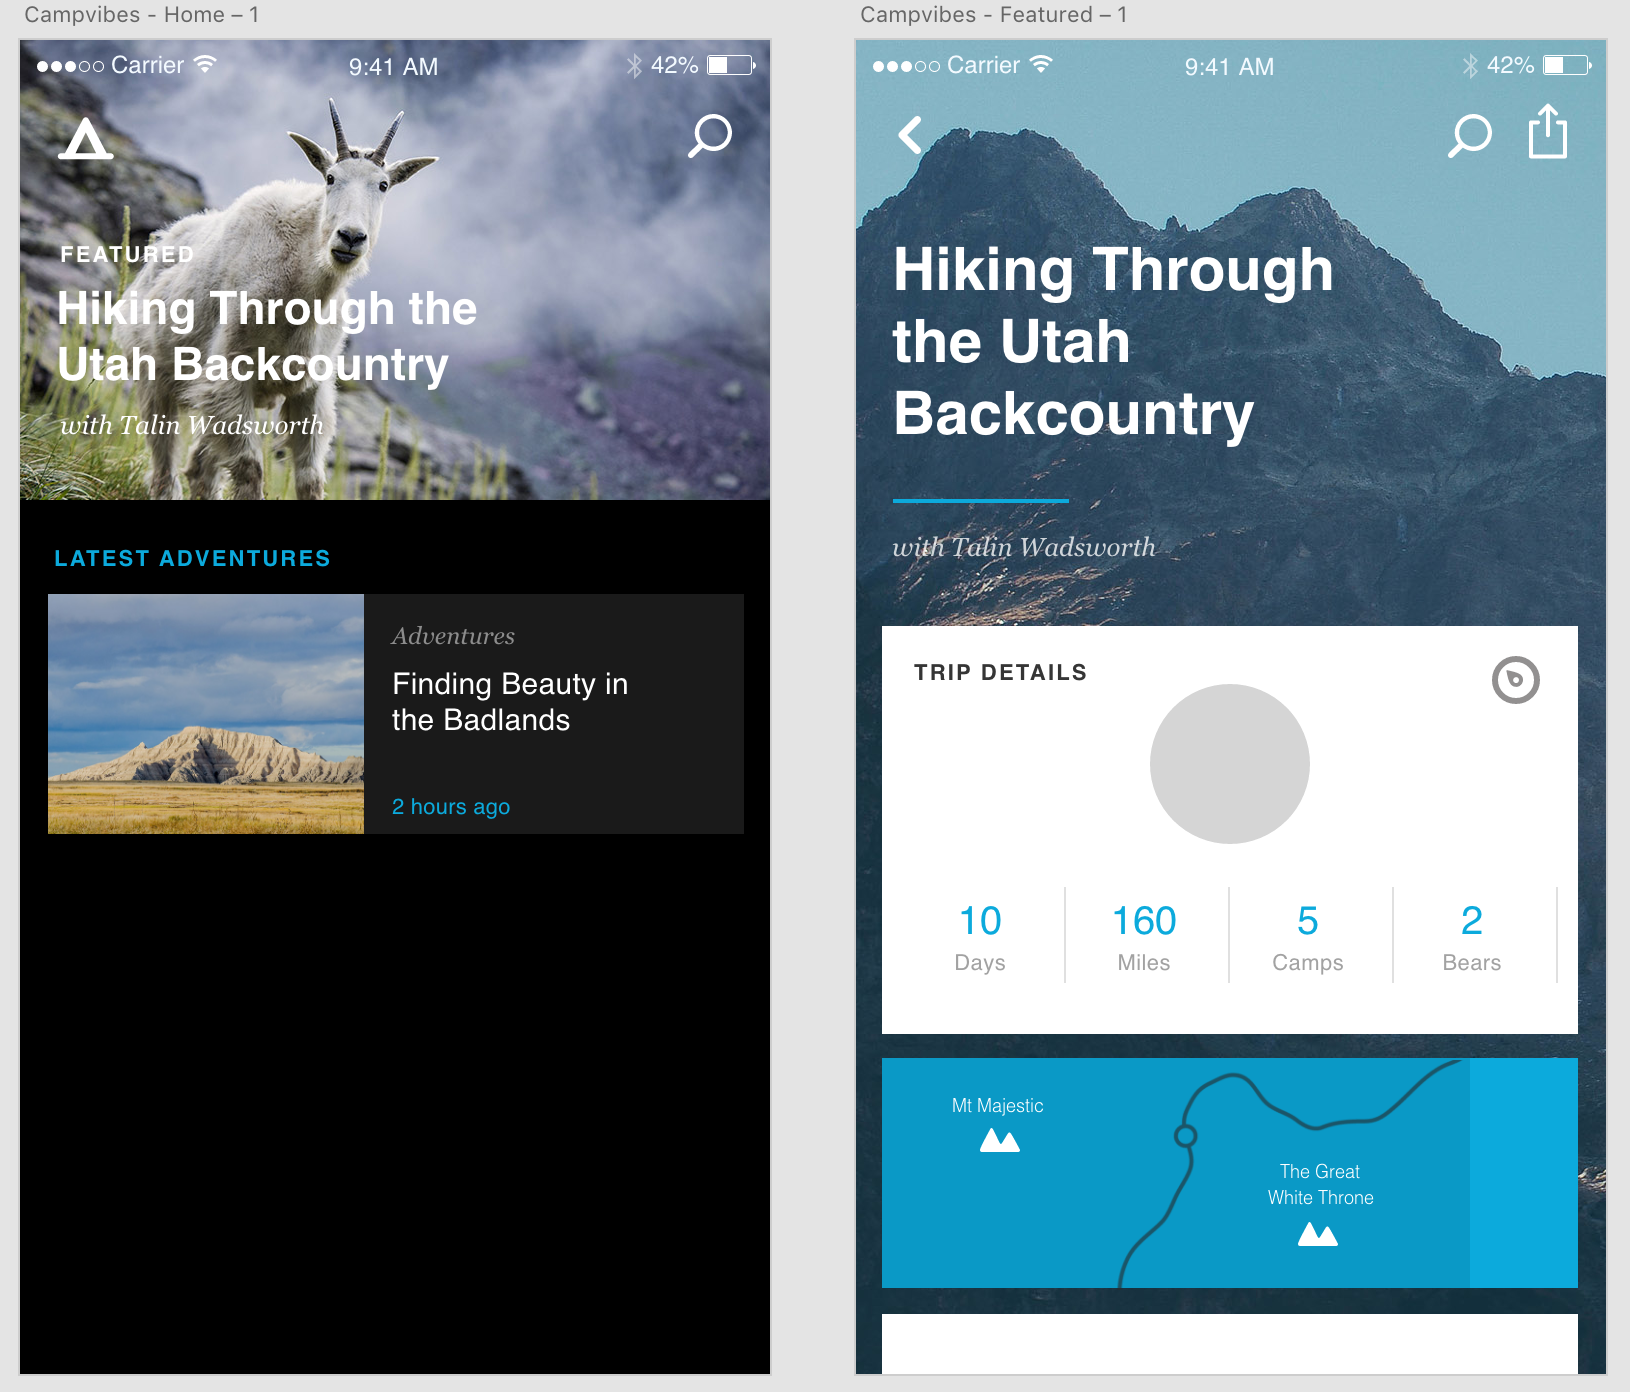
\includegraphics[width=.40\textwidth]{src/img/xd.png}};
\node (solutie) at (7, 0) {BlackBox Soluție};
\node (xcode) at (7, -5) {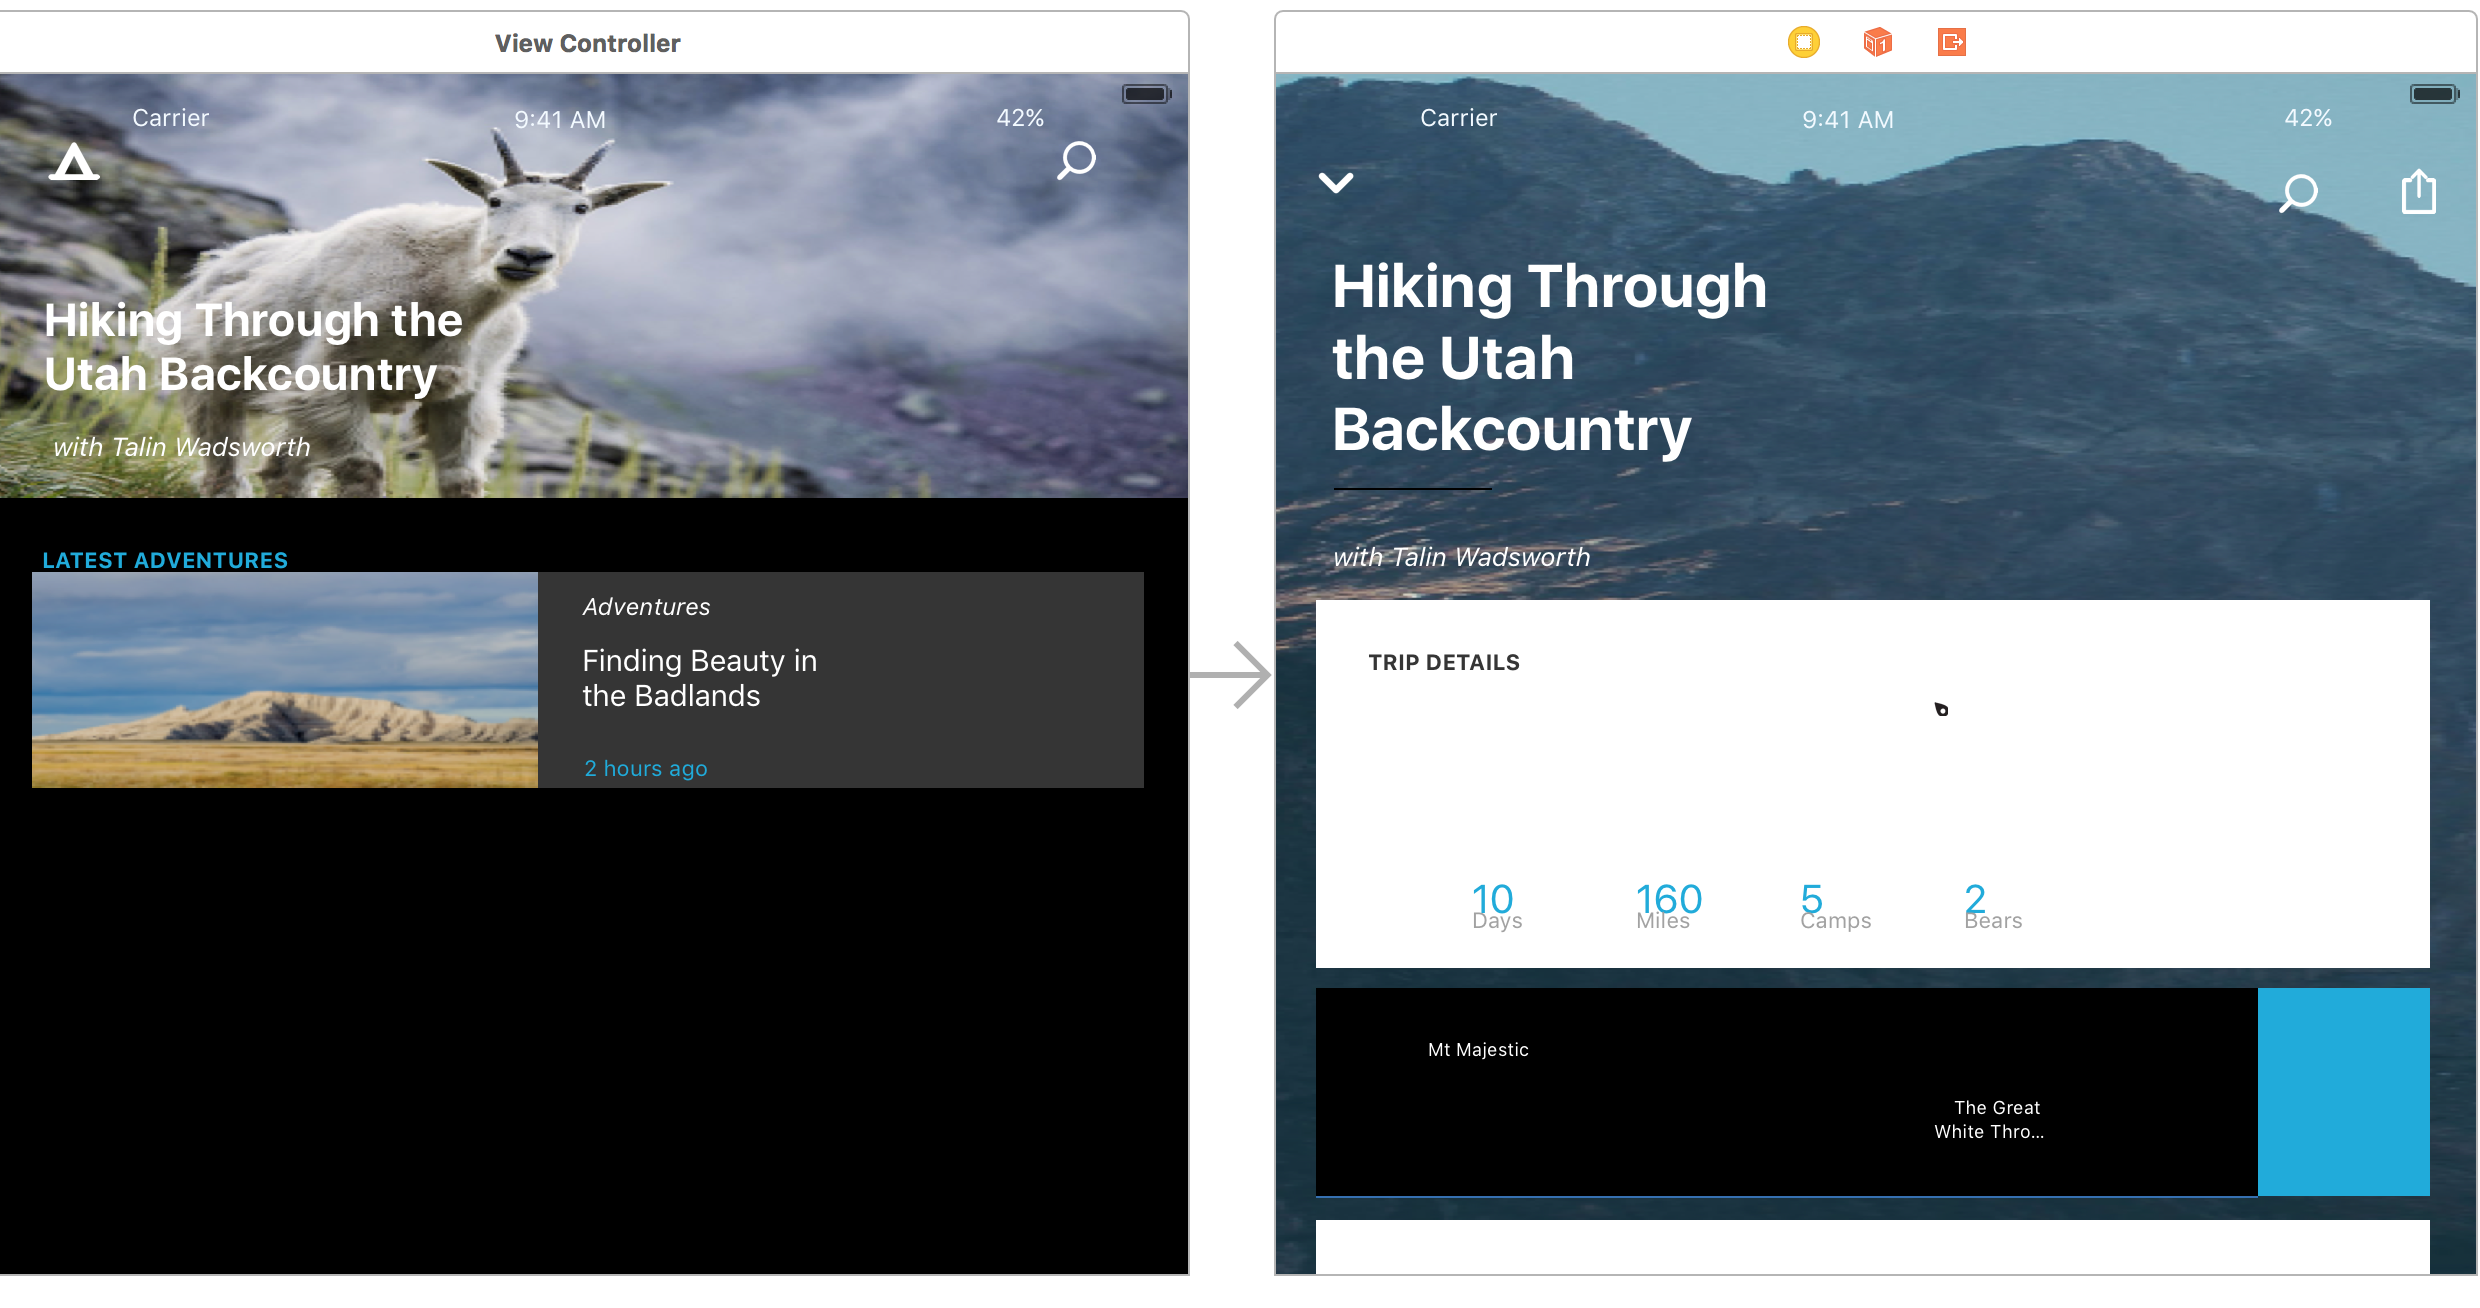
\includegraphics[width=.50\textwidth]{src/img/xcode.png}};
\path (xd.east) -- (solutie.north east) (a1);
\path (solutie.west) -- (solutie.north west) (b1);
\draw [latex-] (solutie) -- (xd);
\draw [latex-] (xcode) -- (solutie);
\end{tikzpicture}
\caption{Prezentare Soluție} \label{fig:Prezentare}
\end{figure}

\subsection{Scop și motivație}
\label{sub-sec:proj-scope}


Finalitatea acestei aplicații este crearea automată  a unei “punți” între două tehnologii dedicate designerilor de UX.

Așadar, principalul scop al acestui proiect este construirea unei scheme de translatare între cele doua reprezentări descrise anterior pentru a veni în ajutorul developerilor de iOS. Prin intermediul soluției descrise, crearea, sincronizarea, actualizarea, dar și colaborarea între membrii unei echipe de dezvolatare de aplicații, se va realiza facil, asigurându-se o automatizare a modului de lucru.

Un scop secundar este găsirea unei soluții eficiente de reprezentare și translatare între cele două tehnologii pentru a fi folosit și în alte domenii de aplicații (baze de date).


\subsection{Obiectivele Proiectului}
\label{sub-sec:proj-objectives}

Obiectivul principal al acestei teme este  acela de translatare între un produs software dedicat dezvoltării unei aplicații (XCode) și o aplicație de design și realizare de prototipuri (Adobe XD). Totodată, prin intermediul acestui proiect se dorește construirea automată a aplicației XCode, pe baza prototipului obținut prin XD.
Astfel, soluția propusă va trebui să asigure următoarele funcționalități:

\begin{enumerate}
\item Soluția va permite unui dezvoltator iOS să creeze un fișier de design Adobe Experience Design care să conțină elementele vizuale din proiectul său iOS (din XCode)
\item Un utilizator poate modifica ecranele aplicatiei, elmentele vizuale și tranzițiile pentru fișierul Adobe Experience Design creat mai sus. De asemenea, se pot crea atât noi elemente vizuale, cât și tranziții.
\item Soluția va permite dezvoltatorului de iOS să-ți actualizeze proiectul său iOS pe baza ultimelor modificări aduse fișierului Adobe Experience Design creat. Sincronizarea se va putea face automat, în momentul în care se salveaza fișierul de design. 
\item  Utilizatorul va putea să compileze aplicația sa iOS din XCode, iar modificările sunt văzute corespunzător. 
\end{enumerate}

De asemenea, un obiectiv secundar al acestui proiect este construirea unei scheme de translatare generică între cele două reprezentări specifice XCode-ului si Adobe XD-ului: xml, respectiv json.
Astfel, soluția propusă se poate extinde, putând fi folosită în diferite domenii de aplicații.


\subsection{Demo}

Aplicația este funcțională și implementează sincronizarea și translatarea directă și inversă a elementelor vizuale dintre Adobe XD și XCode. 
Realizarea proiectului a fost testată pe un sistem MacOSX, aplicația fiind scrisă în ObjC cu ajutorul IDE-ului XCode. Pentru rularea aplicației este necesar proiectul curent  și , desigur, aplicația Adobe XD.
Intern, proiectul se folosește de utilitarul ImageMagick pentru conversia între un format svg și un format png.


\chapter{Prezentarea schemelor de reprezentare}

Așa cum s-a precizat în secțiunile anterioare, proiectul reprezintă un plug-in adus aplicației Adobe Experience Design, pentru interacțiunea cu IDE-ul XCode. 

În acest capitol se va descrie modul de lucru și reprezentările corespunzătoare celor două reprezentări XCode, respectiv XD.

\subsection{Managementul elementelor vizuale in XCode}

XCode este un IDE realizat de Apple care conține o serie de tool-uri pentru dezvoltarea de software pentru OS X, iOS, WatchOS și tvOS. XCode suportă cod sursă pentru o serie de limbaje de programare (C, C++ , Objective-C, Objective-C++, etc.), dar și pentru o serie de modele de programare (Cocoa, Carbon, Java, etc.). Aplicația principală a suitei este IDE-ul, numit de asemenea XCode. Suita XCode include pe lângă documentația Apple de dezvoltare și o aplicație built-in - Interface Builder, o componentă principală in dezvoltarea soluției propuse.

Interface Builder este o aplicație de development de software pentru sistemul Apple Mac OS X, care permite dezvoltatorilor de Cocoa și Carbon să creeze interfețe pentru aplicații folosind interfață grafică. Interfața rezultată va fi stocată într-un fișier .nib (NeXT Interface Builder), sau .xib.

Interface Builder oferă palete de culori, colecții de elemente vizuale - text, tabele, meniuri, butoane, etc - necesare dezvoltatorilor de aplicații ObjC. Astfel , prin intermediul editorului Interface Builder, crearea interfeței grafice pentru utilizator se realizează ușor, fără a fi nevoie de cod efectiv. La baza managementului de elemente vizuale se află Drag & Drop spre canvas-ul de lucru. 

Deoarece Cocoa și Cocoa Touch sunt construite folosind modelul Model-View-Controller, interfețele utilizator se pot realiza independent de implementările lor. Aceste interfețe vor fi stocate în fișierele .nib, iar la compilare, se vor crea dinamic legăturile între UI și implementare.

O aplicație iOS este compusă din multiple scene între care un utilizator navighează. Relațiile dintre aceste scene sunt definite de fișierele .storyboard, care vor reprezenta întregul flow al aplicației. Prin intermediul Interface Builder, storyboard-ul este actualizat conform elementelor grafice afișate, prin crearea, modificarea și realizarea trazițiilor dintre scene.

XCode permite o serie de controllere pentru storyboard: Table View Controller, Collection View Controller, Navigation Controller, Tab Bar Controller, Page View Controller, GLKit View Controller sau Custom View Controller, însă pentru acest proiect soluția propusă rezolvă doar controllerul generic - View Controller. Pentru extinderea acestei soluții și pentru alte tipuri de controllere, va trebui extinsă schema de translatare care va fi prezentată ulterior, conform specificațiilor.

\subsubsection{Anatomia unui fișier .storyboard}

În această secțiune se va explica anatomia de bază al fișierului .storyboard XML și a câtorva tag-uri principale: \textbf{\textit{scene}}, \textbf{\textit{viewController}}, \textbf{\textit{view}}, \textbf{\textit{segue}}. De asemenea se vor explica modul de interacțiune între entități și modul în care acestea lucrează impreună pentru construirea interfețelor utilizator din Interface Builder.
Un fișier “.storyboard” mapează elementele vizuale într-o reprezentare de tip xml. Așadar, fiecărui element vizual îi corespunde un tag cu atribute care specifică carcateristicile acestuia în mod formal. Întrucât tagurile au o reprezentare ierarhică, atributele acestora depind de tag-urile părinte. De exemplu, un tag de încadrare al unui element vizual este definit relativ la tagurile sale părinte de încadrare.

În momentul în care un nou storyboard este creat, se va construi un fișier xml cu tag-ul părinte \textbf{\textit{document}} și cu o serie de atribute care conțin informație meta:


\lstset{language=XML}
\begin{lstlisting}
<?xml version="1.0" encoding="UTF-8" standalone="no"?>
<document type="com.apple.InterfaceBuilder3.CocoaTouch.Storyboard.XIB" version="3.0" toolsVersion="7706" systemVersion="14E46" targetRuntime="iOS.CocoaTouch" propertyAccessControl="none" useAutolayout="YES" useTraitCollections="YES">
  <dependencies>
    <plugIn identifier="com.apple.InterfaceBuilder.IBCocoaTouchPlugin" version="7703"/>
  </dependencies>
  <scenes/>
</document>
\end{lstlisting}

Atributul \textbf{targetRuntime}  specifică sistemul de runtime în care storyboard-ul este folosit. \textbf{\textit{iOS.CocoaTouch}} specifică faptul că storyboard-ul este de tipul iOS.

Tag-ul \textbf{dependencies} identifică orice dependență necesară storyboard-ului. Tag-ul copil \textbf{plugin} specifică pluginul necesar acestui storyboard.

Tag-ul \textbf{scenes} conține toate scenele (view controllers) din storyboard. Reprezentarea xml corespunzătoare este de forma: 

\lstset{language=XML}
\begin{lstlisting}
<scene sceneID="TZ1-Tx-w3d">
  <objects>
    <viewController id="Z5v-SE-Hvj" sceneMemberID="viewController">
      <layoutGuides>
        <viewControllerLayoutGuide type="top" id="y7V-kb-M9q"/>
        <viewControllerLayoutGuide type="bottom" id="GgS-WF-AQQ"/>
      </layoutGuides>
      <view key="view" contentMode="scaleToFill" id="0q9-ar-rJW">
        <rect key="frame" x="0.0" y="0.0" width="600" height="600"/>
        <autoresizingMask key="autoresizingMask" widthSizable="YES" heightSizable="YES"/>
        <color key="backgroundColor" white="1" alpha="1" colorSpace="calibratedWhite"/>
      </view>
    </viewController>
    <placeholder placeholderIdentifier="IBFirstResponder" id="sPm-3H-Ntc" userLabel="My Responder" sceneMemberID="firstResponder"/>
  </objects>
  <point key="canvasLocation" x="426" y="370"/>
</scene>
\end{lstlisting}

Reprezentarea sub formă de arbore a blocurilor XML este de forma:

\begin{tikzpicture}
\treeroot{scene}
\treeentry{objects}{1}
\treeentry{viewController}{2}
\treeentry{viewControllerLayoutGuide}{3}
\treeentry{view}{3}
\treeentry{rect}{4}
\treeentry{autoResizingMask}{4}
\treeentry{color}{4}
\treeentry{placeholder}{3}
\treeentry{point}{1}
\end{tikzpicture}

Un atribut important de menționat ar fi \textbf{id}, atribut prezent în aproape taote tagurile. Atributul \textbf{id} specifică un număr de ordine unic pentru fiecare entitate din storyboard, 
astfel fiecare relație sau conexiune se referă la acest id.

În momentul în care se adaugă o noua scenă, se creează un tag copil \textbf{\textit{scene}} în cadrul tagului \textbf{\textit{scenes}} în storyboard. Tag-ul point specifică offsetul scenei în cadrul canvas-ului de lucru.

Tag-ul \textbf{viewController} reprezintă View Controller -ul principal. Reprezentarea sa xml este de forma:

\lstset{language=XML}
\begin{lstlisting}
 <viewController id="1C9CF5D3-1A5A-41C4-BC52-F3977FC9F164" customClass="ViewController" sceneMemberID="viewController">
\end{lstlisting}

Fiecare View Controller conține o scenă principală și este reprezentată de tag-ul \textbf{view} . 

\lstset{language=XML}
\begin{lstlisting}
<view key="view" contentMode="scaleToFill" id="0q9-ar-rJW">
    <rect key="frame" x="0.0" y="0.0" width="600" height="600"/>
    <autoresizingMask key="autoresizingMask" widthSizable="YES" heightSizable="YES"/>
    <color key="backgroundColor" white="1" alpha="1" colorSpace="calibratedWhite"/>
    <color key="tintColor" white="0.33333333333333331" alpha="1" colorSpace="calibratedWhite"/>
</view>
\end{lstlisting}

Proprietățile unei scene sunt reprezentate, așa cum se vede în xml-ul de mai sus, prin tagurile \textbf{rect}, \textbf{color}, iar atributul \textbf{key} specifică cartacteristica pe care tag-ul curent o definește.

În momentul în care adaugă view-uri copil la view-ul părinte, așa cum se vede în figura alăturată:

\labelindexref{Figure}{img:report-framework} , 

\fig[scale=0.5]{src/img/views.png}{img:report-framework}{Views tag}

reprezentarea xml asociată va fi de forma :
\lstset{language=XML}
\begin{lstlisting}
<view key="view" contentMode="scaleToFill" id="0q9-ar-rJW">
   ...
    <subviews>
        <label opaque="NO" userInteractionEnabled="NO" contentMode="left" text="Label" lineBreakMode="tailTruncation" baselineAdjustment="alignBaselines" id="ngq-9d-cwY">
            <rect key="frame" x="279" y="129" width="42" height="21"/>
            <color key="textColor" red="0.0" green="0.0" blue="0.0" alpha="1" colorSpace="calibratedRGB"/>
            <nil key="highlightedColor"/>
        </label>
        <button opaque="NO" contentMode="scaleToFill" fixedFrame="YES" ... id="mce-tZ-GZN">
            <rect key="frame" x="277" y="201" width="46" height="30"/>
            ...
        </button>
    </subviews>
</view>
\end{lstlisting}

Toate proprietățile setate pentru un UIView, oricare ar fi el - buton, text, imagine, etc. - se translatează automat în atribute sau taguri în fișierul xml.

În momentul în care un două view controllere se conectează cu un segue, un tag numit \textbf{connections} este creat și este inclus în interiorul tag-ului \textbf{viewController}.

Tag-ul \textbf{segues} reprezintă tranzițiile între view controllere sau butoane și alte view controllere.

\lstset{language=XML}\label{segueXML}
\begin{lstlisting}
 <viewController id="Z5v-SE-Hvj" customClass="MyViewController" sceneMemberID="viewController">
                    ...
                    <connections>
                        <segue destination="tr7-0U-dbu" kind="show" identifier="Segue_ShowSecondViewController" id="bCn-xA-8eX"/>
                    </connections>
                </viewController>
}
}
\end{lstlisting}

Tag-ul \textbf{segue} definește atributele \textbf{destination} și \textbf{kind}. Atributul \textbf{destination} specifică \textbf{id}-ul View Controllerului către care se duce tranziția, iar \textbf{kind} specifică tipul tranziției (show sau modal).

View Controllerele pot avea mai multe tranziții și pot pointa către mai multe view controllere. Acest lucru este specificat prin multiple tag-uri \textbf{segue}.

\subsubsubsection{Formatul xml}

XML (Extensible Markup Language) este un limbaj care definește un set de reguli pentru codificarea documentelor într-un format atât human-readable, cât și machine-readable. 

Scopul XML-ului este acela de furnizare de simplicitate, uzabilitate și generalitate în cadrul Internetului. XML-ul este un limbaj care este folosit în cadrul a numeroase aplicații. Acesta a stat la baza protocoalelor de comunicatie, cum ar fi XMPP. De asemenea, aplicațiile pentru Microsoft .NET Framework folosesc fișiere xml de configurare. În cadrul fișierului xd pe care îl vom studia în capitolul următor, metadata de configurare este stabilită tot prin limbajul xml. 

Schema de translatare propusă în acest proiect a fost folosită și în cadrul acestor fișiere de configurare din xd.

\subsection{Managementul elementelor vizuale in XCode}

Adobe Experience Design este un nou utilitar pentru realizarea designului și prototipului de aplicații dedicate UX. Adobe XD este o soluție all-in-one care îi permite unui dezvoltator de iOS să creeze aplicații mobile și website-uri. 

\subsubsection{Anatomia unui fișier .xd}

În urma realizării unei aplicații Adobe Experience Design, se creează un fișier cu extensia .xd, care va conține reprezentarea elementelor vizuale. 
Un fișier xd este realizat prin comprimarea mai multor fișiere de metadata cu extensia “.agc”, prin realizarea operației de zip. Fișierele cu extensia .agc conțin informații legate de scenele din XD în format json.

Ierarhia de fișiere din cadrul unui design .xd (în urma aplicării comenzii unzip) este de forma:

\begin{figure}[!htbp]
\begin{tikzpicture}
\treeroot{.}
\treeentry{META-INF}{1}
\treeentry{metadata.xml}{2}
\treeentry{artwork}{1}
\treeentry{artboard-artboard1}{2}
\treeentry{graphics}{3}
\treeentry{graphicContent.agc}{4}
\treeentry{artboard-artboard2}{2}
\treeentry{graphics}{3}
\treeentry{graphicContent.agc}{4}
\treeentry{interactions}{1}
\treeentry{interactions.json}{2}
\treeentry{manifest}{1}
\treeentry{mimetype}{1}
\treeentry{resources}{1}
\treeentry{2007e145a4a2ade85c55f607adf5a89a}{2}
\treeentry{5348e3c71d48b8267507615bfea3b749}{2}
\treeentry{graphics}{2}
\treeentry{graphicContent.agc}{3}
\end{tikzpicture}
\caption{Ierarhie fișiere} \label{fig:ierarhie}
\end{figure}

Fișierul \textbf{metadata.xml} conține metadata referitoare la fișierul .xd - data de creare, de modificare, și id-urile canvas-ului.

Directorul \textbf{artwork} conține o serie de fișiere cu informații în format json despre elementele vizuale ale fiecărei scene\footnote{Se vor folosi termenii scene și artboard interschimbabil} în parte. 

Directorul  \textbf{resources} conține o serie de imagini folosite în designul XD, salvate local sub numele id-ului corespunzător. De asmenea, în cadrul acestui director se află informații legate de offet-urile și dimensiunile scenelor.

Directorul \textbf{interactions} conține informații legate de tranzițiile dintre scene.

Fișierul \textbf{manifest} conține metadata referitoare la ierarhia de componente grafice din cadrul fișierului XD. 

Fișierul  \textbf{mimetype} definește aplicația corespunzătoare XD-ului.

Un fișier de descriere a unei scene este reprezentat printr-o serie de proprietăți:  \textbf{version} - specifică versiunea agc-ului, \textbf{resoures}, respectiv \textbf{artboards} fac legătura cu restul fișierelor de descriere. Proprietatea  \textbf{children} descrie lista de elemente vizuale ale scenei, precizând, astfel, pentru fiecare entitate, carcateristicile specifice, cadranul de încadrare și offsetul față de ierarhia de elemente față de care depinde.

\subsubsubsection{Formatul json}

JSON (numit și JavaScript Object Notation) este un format care folosește text human-readable pentru transmiterea obiectelor formate din perechi <cheie, valoare>. De aceea formatul JSON se poate serializa și deserializa ușor în structura de date dicționar.

Un dicționar declară programatic obiectul care realizează asocieri între chei și valori. O pereche cheie-valoare din dicționar se numește un ``entry". În interiorul dicționarului, cheile sunt stringuri unice, nenule. Tipul valorii nu are restricții, în afară de imposibilitatea declarării unei valori nule.

\chapter{Prezentarea schemelor de translatare}

În acest capitol se va prezenta modul de translatare între cele două reprezentăriȘ XCode și XD sau, xml, respectiv json. 

Formatul json este similar xml-ului prin faptul că amandouă reprezentările descriu structuri de date și obiecte serializabile. Multiple protocoale bazate pe xml reprezintă aceleași structuri de date ca json-ul, în mod interschimbabil.

Găsirea unei scheme de translatare între cele două reprezentări se rezumă așadar la găsirea multiplelor mapări între tag-urile și atributele xml-ului, respectiv json-ului. De asemnea, anumite dependențe variază în funcție de aplicarea anumitor aplicații față de anumite atribute sau taguri.

Asocierele dintre tagurile xml și json se află într-o relație one-to-one, de aceea schema de translatare trebuie să fie bidirecțională.

\subsection{Translatarea din XCode în Adobe Experience Design}

Importul elementelor vizuale din XCode în XD presupune parcurgerea fișierelor “storyboard” și inspectarea tagurilor cu atributele corespunzătoare. În urmă inspectării, trebuie să se obțină o reprezentare de tip json a fișierului de intrare.  De aceea, schema de translatare pe care o propun este descrierea unui model de asociere între tagurile xml și elementele json, schemă reprezentată, la rândul său, de un fișier .json.  

Această schemă va fi reprezentată într-un format json datorită caracteristicilor specifice acestui format: reprezentare human-readable, extensibilitate, serializabilitate, deserializabilitate rapidă în și dintr-un dicționar. Un astfel de dicționar asigură accesul la valori într-un timp constant.

Schema de translatare din xml în json a avut parte de două versiuni. 

Prima versiune se bazează pe reprezentarea fiecărei proprietăți din json sub o formă ușor de extins și eficientă din punct de vedere computațional. În acest sens, m-am folosit de mapări <cheie, valoare> care să reprezinte proprietățile și valorile corespunzătoare.

Aceste mapări corespund unor serii de dicționare care reprezintă template-urile elementelor json (formatul în care vrem să translatăm). Așadar, schema propusă va fi construită dintr-un dicționar de template-uri specifice diferitelor proprietăți. 

Fiecare cheie din acest dicționar principal reprezintă numele unei proprietăți din json, iar valoarea corespunzătoare - template-ul proprietății json. 

Pe lângă acest dicționar - pe care o sa îl numim \textbf{rootDict} - avem nevoie de o mapare între tagurile xml și proprietățile json care specifică același element vizual/ logic. Pentru aceasta, ne folosim de un dicționar de mapare suplimentar care va fi sub forma (<nume_tag_xml>,  <nume_proprietate_json>). Pe acest dicționar îl vom numi în continuare \textbf{mapDict}.

Așadar, prin intermediul celor două dicționare rezolvăm problema mapării dintre cele două reprezentări. Apare, însă altă problemă: cum rezolvăm legăturile dintre proprietăți ?

De exemplu, fie figurile \todo{2 figuri} care reprezintă un text în XCode, respectiv în XD.
Proprietățile care variază - dimensiunile cadranului (\textbf{rect}), culorile (\textbf{color} cu atributele \textbf{fontDescription} și \textbf{background}), textul efectiv (atributul \textbf{text}) - vor trebui să fie înlocuite corespunzător în template-ul de json.
De aceea introducem niște notații care ne ajută în realizarea acestor asocieri. 


\newtheorem{mydef}{Definiție}[chapter]
\newtheorem{myNote}{Notă}[chapter]

\begin{mydef}\label{dollar}
Un string precedat de caracterul ``\$" reprezintă o valoare care trebuie să fie înlocuită, conform comportamentului definit de acesta.
\end{mydef}

\begin{mydef}\label{dot}
Un string care are în compoziția sa caracterul ``." reprezintă nivelele de indirectare într-o reprezentare json sau xml. Fiecare substring precedat de ``." reprezintă un nou nivel de indirectare al unui format care poate fi transformat într-un dicționar - pe care îl vom numi \textbf{generalDict} .
\end{mydef}

\begin{mydef}\label{count}
Fie string-ul ``x1.x2. ... .xn" care respectă definiția \ref{dot}. Împărțim stringul inițial în mai multe substringuri delimitate de ``." și obținem un vector de substringuri de dimensiune n. Acest vector va avea următoarea proprietate: primele n-1 substringuri sunt chei în dicționarul \textbf{generalDict} prezentat în definiția \label{dot}. 
\end{mydef}

\begin{mydef}
Toate definițiile de mai sus sunt valabile și în cazul aplicării acestora simultan (pentru același string).
\end{mydef}

\begin{figure}[!htbp]
\begin{lstlisting}[language=json,firstnumber=1]
{"textField" : {
        "type" : "text",
        "name" : "$text",
        "transform" : {
            "a" : "1",
            ...
            "tx" : "$rect.x",
            "ty" : "$rect.y"
        },
        "style" : {
            "fill" : {
                "type" : "solid",
                "color" : {
                    "mode" : "RGB",
                    "value" : {
                        "r" : "$color.red",
                        "g" : "$color.green",
                        "b" : "$color.blue"
}

\end{lstlisting}
\caption{Schemă translatare xcode->xd} \label{fig:XCode2XD Schema}
\end{figure}

Pentru a exemplifica definițiile de mai sus, ne vom folosi de figura \ref{fig:XCode2XD Schema} și de string-urile \$color.red, \$text. 

Procedeul de aplicare al definițiilor este următorul:


\begin{itemize} \label{modalitate}
\item Pentru \$color.red (cheia ``r"): 
\begin{enumerate}
\item Observăm că stringul este o valoare temporară (care va trebui să fie înlocuită) conform definiției \ref{dollar}
\item Evaluam valoarea stringului; Observăm că stringul este de tipul definiției \ref{dot}
\item Împărțim stringul color.red într-un vector de substringuri delimitate de ``." => generalDict = [color, red] unde n = |generalDict| = 2
\item Vectorul ne spune faptul că primele n-1 substringuri din generalDict vor fi chei, iar ultimul substring va reprezenta valoare (conform definiției \ref{count}); Așadar, \$color.red va fi înlocuit cu valoarea găsită la atributul ``red" al tagului ``color".
\end{enumerate}
\end{itemize}


\begin{mydef}\label{cale}
O cale reprezintă nivelele de indirectare din cadrul unui dicționar, relative la o valoare.
Reprezentarea unei căi este realizată prin concatenarea cheilor în drumul spre valoarea dorită, delimitate prin ``.".
\end{mydef}


\begin{mydef}

Un dicționar ``invers" se definește relativ la un alt dicționar. 
Fie dicționarul ``invers" I, iar dicționarul principal P. 
Fie o valoare de forma ``\$x1.x2. ... .xn" într-un nivel oarecare np în cadrul P. 
Fie calea asociată acestei valori de forma ``c1.c2. ... .cn".
Atunci I va conține o valoare egală cu ``c1.c2. ... .cn".
\end{mydef}

\begin{myNote}
Construirea fișierului json final se realizează într-un dicționar pe care o sa îl numim \textbf{resultDict}.
\end{myNote}

Am stabilit, așadar modul în care reprezentăm mapările, dar cum facem efectiv aceste asocieri ? Prin folosirea unui dicționar ``invers" care va fi stocat tot în \textbf{mapDict} așa cum se poate vedea în figura \ref{fig:MapDict Schema}.

\begin{figure}[!htbp]
\begin{lstlisting}[language=json,firstnumber=1]
{"imageView."    :   "style.fill.pattern.href",
    "rect." : {
        "x" :   "textField.transform.tx",
        "y" :   "textField.transform.ty",
        "width" : {
            "rect"  :   "rect.shape.width",
            "text"  :   "textField.shape.width",
            "shape" :   "imageView.style.fill.pattern.width"
        
        },
        "height" : {
            "text"  :   "textField.shape.height",
            "rect"  :   "rect.shape.height",
            ...
}
\end{lstlisting}
\caption{Schemă translatare mapDict} \label{fig:MapDict Schema}
\end{figure}


Dicționarul invers ne va ajuta să găsim, pentru un anumit tip de element xml, proprietățile care trebuie înlocuite și să facem această modificare. 

Algoritmul pentru această metode este următorul:

\begin{enumerate}
\item Pentru a realiza o separare între cod și schemele de translatare, acestea vor fi stocate în fișiere separate, care la pornirea aplicației, vor fi încărcate în memorie.
\item Se parcurge fișierul storyboard asociat aplicației XCode prin intermediul clasei NSXMLParser. Pe măsură ce se parcurge fișierul, obținem numele tagului curent și un dicționar cu atributele și valorile asociate.
\item Verificăm dacă există vreo numele tagului curent apare în dicționarul mapDict
\begin{itemize}
\item \textbf{Cazul Adevarat}: Valoarea mapării găsite reprezintă denumirea proprietății în XD. Fie această valoare X. Se găsește entry-ul din dicționarul rootDict care are cheia egală cu X. Valoarea entry-ului va reprezenta template-ul elementului vizual în reprezentarea XD și va fi adăugat la rootDict.
\item \textbf{Cazul Fals}: Tagul curent reprezintă o caracteristică de la care trebuie să preluam anumite informații. De aceea, căutăm în dicționarul invers numele tagului și obținem o valoare X. Valoare respectivă poate fi de două tipuri:
\begin{itemize}
\item string : caz general, calea către obiectul care trebuie înlocuit este similară pentru orice tagș Se parcurge calea definită sub forma ``c1.c2. ... .cn" (conform definiției \ref{cale}) din dicționarul rootDict; Se obține o valoare Y sub forma ``\$x1.x2. ... .xn"; În continuare se procedează similar algorimtului din \ref{modalitate}.
\item dicționar :
\end{itemize}
\end{itemize}
\end{enumerate}


Cea de-a doua metodă de translatare va explica ulterior, după translatarea din XD în XCode, din cauza unor noțiuni specificate în cadrul acelui capitol.

În urma obținerii dicționarului json, există două posibilități. În primul rând, dicționarul obținut se poate copia în Clipboard (prin intermediul clasei NSPasteboard), urmând ca apoi, în urma unui acțiuni de Cmd + V în scena XD, să se copieze elementele vizuale în fișierul de design.

A doua modalitate este reprezentată de construirea ierarhiei de fișiere prin împărțirea fiecărei scene într-un fișier separat. De asemenea trebuie generate automat id-uri unice în cadrul aplicației pentru fiecare element, fie el logic, sau vizual. Fișierul manifest va conține ierarhia de fișiere, descrisă în json, extinsă prin caracteristici precum id unic, cale către fișiere din ierarhie și dimensiune.



\subsubsection{Translatarea Switch-ului și a altor elemente grafice similare}

Un switch permite utilizatorului pornirea sau oprirea rapidă a unor opțiuni mutual exclusive. 
Interface Builder are un obiect de tip Switch care poate fi ușor adăugat aplicației. XD-ul, însă, nu are un element de sine stătător care să reprezinte un astfel de element vizual. Există librării care au construite anumite elemente vizuale (cum ar fi butonul, slider-ul, etc.) dar care descriu segmentele din care este alcătuit assetul. 

De aceea, pentru translatarea acestor obiecte, se creează un fișier care conține template-ul obiectului respectiv din XD. Pentru modificarea caracteristicilor (dimensiuni cadran, culoare, etc.), se vor folosi schemele de translație, similar algoritmului prezentat anterior.

\subsubsection{Translatarea Interacțiunilor XCode->XD}

O interacțiune în XCode, denumită ``segue", este o conexiune care reprezintă tranziția dintre o scenă A și o altă scenă B. Relațiile și conexiunile sunt reprezentate vizual printr-o săgeată de la scena expeditor, la scena destinație. În mijlocul acestei săgeți se află o formă care specifică tipul de segue. Tipurile de segue se pot vede în figura \ref{img:segue}. Soluția propusă are suport doar pentru Show segue.

\labelindexref{Figure}{img:segue}

\fig[scale=0.5]{src/img/segue.png}{img:segue}{Switch tag}

O interacțiune între un element vizual și o scenă se realizează prin intermediul id-urilor unice, specifice fiecărui asset. Acest lucru este valabil atât în XCode, cât și în XD. De aceea este nevoie o mapare între un id și elementul vizual pe care îl specifică. 

Astfel, soluția propusă implementează un dicționar cu mapări <id_unic, array> (pe care îl vom numi \textbf{segueDict}), unde array reprezintă un vector de doua obiecte. Primul obiect este reprezentat de numărul scenei din care face paret assetul, iar al doilea - numărul de ordine al elementului vizual din scenă.

De asemenea, trebuie reținut ultimul id întalnit. Așa cum se vede în figura \ref{segueXML}, interacțiunea depinde de id-ul destinație (tr7-0U-dbu) și de id-ul elementului vizual curent (Z5v-SE-Hvj). Acesată mapare se va adăuga unui dicționar (pe care îl vom numi \textbf{segueDict})care va conține toate interacțiunile de pe canvas.

Pentru construirea interacțiunilor în XD, toate id-urile stocate în dicționarul \textbf{segueDict} trebuie să fie adăugate elementelor vizuale corespunzătoare, conform regulilor de mapare din dicționarul \textbf{segueDict}.

Mapările din \textbf{segueDict} vor fi copiate în cele din urmă în fișierul interactions.json.

\subsection{Translatarea din Adobe Experience Design în XCode}

\todo{adobe -> text frame porneste din stanga jos; xcode -> text frame porneste din stanga sus}

Exportul elementelor vizuale din Adobe XD în Xcode presupune parcurgerea fiserelor “agc”  și inspectarea elementelor acestuia. Particularizarea problemei presupune găsirea schemei de translatare de la un format de tip json la un format de tip xml. Așa cum s-a precizat în secțiunea anterioară, maparea XD-Xcode este o mapare complexă de tip one-to-one, care se bazează pe moștenire și  aplicare de operații. 

Schema propusă pentru export se poate extinde pentru translatarea dintre json și xml pentru orice fel de aplicație, prin respectarea câtorva reguli explicate mai jos. 

Pentru implementarea acestei scheme se vor folosi două dicționare cu mapari ale celor două limbaje.  În primul rând, anumite elemente json sunt în relație de echivalentă cu anumite taguri xml. 


\begin{mydef}\label{echivalent}
Numim relație de echivalentă, relația în care cele două entități din json, respectiv din  xml reprezintă același obiect vizual (sau logic). 
\end{mydef}

\begin{myNote}\label{tip}
Tipul oricărui element din XD este specificat prin proprietatea ``type", care există în cadrul oricărei reprezentări json al unui asset. De exemplu, pentru text, tipul se numește tot ``text";
\end{myNote}

\begin{myNote}\label{echivalent}
Proprietatea ``type" din cadrul unei reprezentări nu specifică de una singură apartenența la o clasă logică de asset; În această categorie intră imaginile; Pentru a specifica apartenența la un anumit tip de asset trebuie îndeplinite o serie de reguli tipice categoriei respective.
\end{myNote}

De exemplu, obiectul vizual “label” corespunzător reprezentării .xml conține ca asociere în .json un obiect caracterizat de tipul “text”. Aplicarea definiției \ref{echivalent} se poate observa în figura \ref{fig:XD2XCode Defs} care va fi stocată într-un prim dicționar \textbf{defDict}.

Se poate observa faptul că acest dicționar conține o serie de mapări de tipul <Key, Value>, unde ``Key" reprezintă valoarea specifică proprietății ``type". ``Value" reprezintă fie un obiect de tip string, fie un obiect de tip dicționar. În cazul în care ``Value" este un string, vom ști faptul că tipul obiectului curent este stabilit prin valoarea lui ``Value". În caz contrar, ``Value" va reprezenta un alt dicționar ale carui chei sunt stringuri de forma \ref{count}. Aceste chei menționate vor reprezenta niveluri de indirectare în dicționarul xd. Toate aceste chei vor reprezenta, la nivel logic, branchuri if-else, care ne ajută la descoperirea categoriei din care face parte assetul curent. În momentul în care, prin parcurgerea nivelelor de indirectare specificate în cheie, vom ajunge la o valoare diferită de null, algoritmul se va aplica pentru noul dicționar obținut. În cele din urmă vom obține categoria din care face parte assetul curent. 

\begin{myNote}\label{tip similar}

Pentru o a numită categorie de asseturi (de ex. pentru shape), pot exista mai multe modele de reprezentare, sau mai multe tipuri de asocieri, În funcție de fișierul .xml.
\end{myNote}

În cazul în care tipul obținut în urma aplicării algoritmului menționat mai devreme, se obține un string de forma definiției \ref{dollar}, atunci acel tip corespunde notei \ref{tip similar}.

De aceea, trebuie să păstrăm și această mapare în dicționarul din figura \ref{fig:XD2XCode Defs}.


\begin{figure}
\begin{lstlisting}[language=json,firstnumber=1]
  {...
  "text"     :   "label",
  "shape"     :   {
        "shape.type.rect" : {
            "style.fill.type.pattern" : "imageView",
            "style.fill.type.solid"   : "$frame"
        },
        "shape.type.path" : {
            "style.fill.type.solid" : "$imageView"
        },
        "shape.type.line" : {
            "style.fill.type.none" : "$lineView"
        }
  ...
\end{lstlisting}
\caption{XD2XCode Defs} \label{fig:XD2XCode Defs}
\end{figure}


Cel de-al doilea dicționar va conține un template al reprezentării în care se va dori translatarea. Acest template este scris într-un format .json, datorită modului facil de reprezentare și extindere. De asemenea, un astfel de format poate fi deserializat intr-un dictionar. Organizarea acestei scheme de translatare .json este realizată după modelul din Figura (2). Tag-urile din xml se pot împarți în trei categorii, în funcție de elementul reprezentat. Categoriile specificate sunt următoarele: content, subViews, subTags. Prin specificarea acestora, se dorește modularizarea implementării și separarea elementelor logice din cadrul proiectului. Fiecare tag, indiferent de categoria în care se află, se va conforma formatului prezentat în Figura(2).  

\begin{figure}
\begin{lstlisting}[language=json,firstnumber=1]
{
"view" : {
        "header": {
            "key" : "view",
            ...
            "toString" : ["key", "contentMode", "id"] },
        "toString" : ["header", "rules"],
        "rules" : { 
            "$header.id" : "$rand",
            ...
            "subviews" : {
                "$children.$sceneNo.artboard.children" : {}},
            "color" : {
                "$children.$sceneNo.style.fill.color.value" : {
                    "red" : "$r",
                    ...
                    "colorSpace" :"calibratedRGB" }},
            "toString" : ["rect", "autoresizingMask", "subviews", "color"],
            "order" : ["$header.id", "rect", "autoresizingMask", "color", "subviews"] }
        .... }
\end{lstlisting}
\caption{XD2XCode Schema} \label{fig:XD2XCode Schema}
\end{figure}

O mapare corectă a unui tag trebuie să corespundă anumitor reguli de compunere și de afișare. De asemenea, construcția unui tag trebuie, în anumite cazuri, să respecte o anumită ordine. Acest lucru este necesar întrucât, în anumite cazuri, regulile de translatare între cele două reprezentări se bazează pe “mostenire”. Această relație garantează faptul că un tag care apare la un nivel inferior, va moșteni atributele părintelui, aka atributele copilului sunt “relative” la atributele părintelui. O bună exemplificare a acestei proprietăți este “mostenirea” cadrului în care se află un părinte. Tag-ul copil (tag care se află la un nivel inferior față de tag-ul de bază) va avea offsetul relativ la cadranul părintelui, iar dimensiunea în care “copilul” va putea fi așezat este dimensiunea spațiului “parinte”. Aceste specificații sunt reprezentate prin adăugarea elementului “order” cu lista de ordine corespunzătoare. 
Dependențele și regulile de mapare vor fi specificate în cadrul elementului json “rules”. Acesta va conține un dicționar cu mapari <Key, Value>, unde Key reprezintă tagul/atributul care va fi modificat, iar Value va reprezenta la rândul său un dicționar de mapari <KeyDep, ValueDep>.  “KeyDep” va reprezenat dependența tagului Key față de valorile “KeyDep”. Maparile explicite sunt specificate în cadrul ValueDep prin mapari de tipul <key_of_tag, value_from_KeyDep>. 
Parsarea și, în cele din urmă afișarea reprezentării în format “xml” va fi specificată prin intermediul tag-ului “toString”. 
De asemenea, trebuie precizată structură de tip “<strîng>.<…>.<strîng>” care reprezintă nivelel ierarhice din cadrul dictionatului care trebuie să fie parcurse. Această reprezentare trebuie să asigure faptul că având o înșiruire de stringuri separate prin punct (n șiruri), n șiruri vor fi chei în dicționarul de translatare. 

\subsubsection{Translatarea Path-urilor și a diverselor figuri geometrice}

Pe măsură ce se desenează în cadrul unei scene, se creează o linie numită \textbf{path}, care este compusă din unul sau mai multe segmente drepte sau curbe care pot fi manipulate cu precizie ridicată.

Un path este reprezentat în XD sub forma unei proprietăți json sub forma:


\begin{tikzpicture}
\treeroot{.}
\treeentry{type:shape}{1}
\treeentry{transform}{1}
\treeentry{...}{2}
\treeentry{tx:100}{2}
\treeentry{ty:100}{2}
\treeentry{style}{1}
\treeentry{fill}{2}
\treeentry{color}{3}
\treeentry{red:255}{4}
\treeentry{...}{4}
\treeentry{stroke}{2}
\treeentry{...}{3}
\treeentry{shape}{4}
\treeentry{path:M 204.35 739.36 C 207.01 739.91 209.11 ...}{5}
\end{tikzpicture}

Se poate observa că informațiile oferite de această reprezentare se pot translata ușor într-un \textbf{svg}. 

Scalable Vector Graphics sau SVG este un format de reprezentare al imaginilor vectoriale 2D bazat pe xml. Reprezentarea internă a unei imagini svg este de forma 
\lstset{language=XML}
\begin{lstlisting}
<svg xmlns="http://www.w3.org/2000/svg" viewBox="447.582 176.598 87.418 92.402">
<defs>
<style>
  .cls-1 {
    fill: #fff;
    stroke: #95989a;
    stroke-width: 1px;
  }
</style>
</defs>
  <path id="rectangle-1" class="cls-1" d="M 204.35  ..." transform="translate(448 177)"/>
</svg>
\end{lstlisting}

Pentru translatarea din formatul json în formatul xml este nevoie de substituirea proprietăților \textbf{viewBox}, \textbf{fill}, \textbf{stroke}, \textbf{d} din \textbf{path} cu caracteristicile din json. 

\textbf{ViewBox} reprezintă cadranul în care path-ul este vizibil. Acesta va fi construit prin găsirea maximului și al minimului pe axele X, respectiv y. Valorile de minim vor reprezenta primele valori din viewBox (offsetul de pornire), iar diferența între minim și maxim pe axele x și y vor reprezenta lățimea și lungimea cadranului.

Valoarea \textbf{path} va conține reprezentarea segmentelor din care forma geometrică este constituită.

În urma translatării, se va obține un fișier svg cu elementul vizual regăsit în xd. 

Din păcate, XCode-ul nu suportă formatul svg, de aceea pentru aducerea acestor asset-uri în aplicația XCode dezvoltată, mai este nevoie de un pas. Pasul constă în transformarea svg-ului într-un format png, suportat de XCode. Această transformare va fi realizată prin comanda convert din cadrul utilitarului ImageMagick. 

Apelul comenzii \textbf{convert} presupune crearea unui NSTask - un subprogram cu imaginea executabila , în cazul de față, \textbf{convert}  care va fi monitorizat de aplicația curentă. 

Similar, se poate construi fișierul svg pentru linii prin adăugarea tag-ului <line ...> în cadrul svg-ului.

\subsubsection{Translatarea grupurilor}

Un grup în XD reprezintă o organizare logică a mai multor asset-uri într-un singur element vizual. În urma acestei conversii, asseturile se vor comporta ca o singură entitate. Se pot aplica operații de translatare sau rotire asupra tuturor elementelor interne. 

Reprezentarea sub forma unui json al unui grup este specificată în figura \ref{fig:Group}. 

\begin{figure}[!htbp]
\begin{lstlisting}[language=json,firstnumber=1]
{
  "type":"group",
  "transform":{
    "a":1,
    ...,
    "tx":1647,
    "ty":40},
    "group":{
      "children":
      [{...}]}}
\end{lstlisting}
\caption{Group} \label{fig:Group}
\end{figure}

Proprietatea ``transform" specifică modul de translatare sau rotire al groupului. Toate elementele care aparțin grupului (dicționarele care aparțin listei ``children" )vor fi modificate conform valorilor lui transform.

În Xcode, noțiunea de group este inexistentă, dar se poate face o asociere grup - view . 
Pentru construirea dimensiunilor view-ului, se va realiza o parcurgere inversă de la elementele constitunte grupului, la dimensiunea grupului. 
Așadar se iterează prin colecția de elemente din grup și se calculează offsetul minim și maxim al axelor x și y pentru fiecare. Cadranul grupului va fi încadrat între offsetul minim al axelor x și y și offsetul maxim al acestora.


\subsubsection{Translatarea imaginilor}

Procesarea imaginilor se realizează similar procesării altor elemente vizuale, cu singura diferență că acestea trebuie importate fizic în aplicația XCode.

De aceea, este nevoie de obținerea căii absolute ale imaginilor care trebuie preluate. 
Obținerea căii absolute se realizează prin 3 metode:

\begin{itemize}  
\item obținerea valorii pentru proprietatea ``href", duce la obțierea căii către imaginea dorită
\item Un fișier xd, după decomprimare, așa cum s-a prezentat în figura \ref{fig:ierarhie} conține un director resources care, pe lângă fișierul de descreiere al scenelor, conține și imaginile din XD. Numele imaginilor sunt reprezentate printr-un id unic, care se regăsește și în fișierul de descriere al XD-ului.
\end{itemize}

În urma obținerii căii absolute ale imaginilor, se face o copie locală a acestora într-un director ``Resources" din cadrul proiectului XCode. Aceste fișiere vor trebui să fie adăugate manual (Drag & Drop) în directorul ``Supported Files" al aplicației.

\subsubsection{Translatarea interacțiunilor}

O interacțiune în XD reprezintă o legătură între un element vizual dintr-o scenă și o altă scenă. Prin interacțiuni, aplicația este animată și se pot realiza tranziții între scene, în funcție de comportamentul descris. 

Pentru a realiza translatarea interacțiunilor, se citește fișierul interaction.json, obținându-se astfel un dicționar cu mapări între id-uri pe care o sa în numim \textbf{segueDict}. 

Următoarea etapă constă în parcurgerea dicționarului cu reprezentarea tutoror scenelor, și obținerea mapărilor între id și elementul vizual curent (mapări stocate într-un dicționar \textbf{mapDict}). În momentul în care se obține un id care există sub formă de cheie în dicționarul segueDict, se adaugă la resultDict, template-ul pentru obiectul de tip interacțiune. 

Deoarece id-urile destinație pot reprezenta scene care încă nu au fost procesate, dicționarul final va trebui să fie parcurs încă o dată pentru înlocuirea id-urilor conform mapDict.

\subsection{Sincronizarea scenelor între cele două reprezentări}

Sincronizarea se referă la modul în care elementele vizuale vor fi updatate în momentul în care se realizează o modificare în proiectul XD, sau în proiectul XCode.
Voi incepe cu prezentarea sicronizării de la XD si Xcode, sincronizarea inversă urmând să fie implementată ulterior.

\subsection{Sincronizarea Adobe Experience Design - XCode}

În momentul în care un fișier XD este modificat, aplicația va fi notificată și va începe căutarea scenelor modificate. Această căutare se bazează pe o pre-salvare atât a offseturilor scenelor din Xcode cât și a sha-urilor acestora. 

Offsetul este necesar deoarece un fișier Xcode conține toate scenele din storyboardul reprezentat.  Scenele nemodificate sunt reprezentate prin scenele care au sha-ul în dicționarul de sha-uri presalvate. Maparea acestui sha este realizat împreună cu numărul de ordine al scenei corespunzător. 
În cazul în care o scenă s-a detectat că fiind modificată se re-generează codul corespunzător (așa cum s-a prezentat în secțiunile anterioare).  La fiecare nouă updatare, dicționarele cu offseturi și cu sha-uri trebuie refăcut. 


\subsection{Implementare}

În acest capitol voi oferi detalii despre arhitectură. De asemnea, voi prezenta o statistică a timpilor de rulare și modele de îmbunătățire ale aplicației.

\subsection{Arhitectură}

  
Managementul elementelor vizuale prezentat în capitolele precedente este implementat integral în Objective C. 

Interacțiunea cu fișierele de design XD s-au realizat în două moduri: prin intermediul Clipboardului și prin crearea ierarhiei de fișiere xd.

În primă etapă, preluarea elementelor grafice din Adobe XD s-a realizat prin intermediul Clipboardului. Astfel, interacțiunea cu artboardurile din XD s-a realizat prin mecanismele de copy și paste ale scenelor.

După translatarea din format XCode în format XD, va rezulta un singur fișier .agc care va conține toate informațiile necesare creării fișierului de design. Conținutul acestui fișier va fi pus în Clipboard cu tipul \textbf{com.adobe.sparkler.design}, care va fi apoi copiat în fișierul xd.

Flow-ul importului prin intermediul Clipboardului se regăsește în figura \ref{fig:Clipboard Import}, iar al exportului, prin intermediul Clipboardului, se regăsește în figura \ref{fig:Clipboard Export}.


\begin{figure}[!htbp]
\centering
\begin{tikzpicture}[node distance = 4cm, auto]
\node [block] (init) {.storyboard};
\node [block, right of=init] (solutie) {Soluție translatare};
\node [block, right of=solutie] (clipboard) {Clipboard};
\node [block, right of=clipboard] (xd) {.xd};
\path [line] (init) -- node {input} (solutie);
\path [line] (solutie) -- node {paste} (clipboard);
\path [line] (clipboard) -- node {output} (xd);
\end{tikzpicture}
\caption{Clipboard Import} \label{fig:Clipboard Import}
\end{figure}

\begin{figure}[!htbp]
\centering
\begin{tikzpicture}[node distance = 4cm, auto]
\node [block] (init) {.xd};
\node [block, right of=init] (clipboard) {Clipboard};
\node [block, right of=clipboard] (solutie) {Soluție translatare};
\node [block, right of=solutie] (storyboard) {.storyboard};
\path [line] (init) -- node {copy} (clipboard);
\path [line] (clipboard) -- node {input} (solutie);
\path [line] (solutie) -- node {output} (storyboard);
\end{tikzpicture}
\caption{Clipboard Export} \label{fig:Clipboard Export}
\end{figure}


În a doua etapă - etapa finala - s-a renunțat la folosirea Clipboardului, în favoarea creării fișierului xd. 
Acest lucru s-a realizat din două motive: În primul rând, folosirea Clipboardului implica un flow mai greoi al aplicației și o interacțiune suplimentară a utilizatorului (overhead adus de copy și paste). Cel de-al doilea motiv implică imposibilitatea copierii tranzițiilor prin Clipboard.

Așadar, pentru preluarea informațiilor din cadrul unui fișier xd, se va realiza decomprimarea acestuia prin apelarea comenzii \textbf{zip}. În urma acestui apel, se vor obține ierarhia de fișiere așa cum a fost descrisă în capitolele 1, respectiv 2.

În urma translatării din XCode în XD, se va construi ierarhia de fișiere care va fi fi apoi comprimată în format .xd. Această comprimare se va realiza prin intermediul comenzii \textbf{zip -r --no-dir-entries <ierarhie fișiere> <design xd>}.

Arhitectura acestui model de lucru se regăsește în figurile \ref{fig:Export}, \ref{fig:Import}.

\begin{figure}[!htbp]
\centering
\begin{tikzpicture}[node distance = 4cm, auto]
\node [block] (init) {.storyboard};
\node [block, right of=init] (solutie) {Soluție translatare};
\node [block, right of=solutie] (clipboard) {Creare ierarhie fișiere .agc};
\node [block, right of=clipboard] (xd) {.xd};
\path [line] (init) -- node {input} (solutie);
\path [line] (solutie) -- node {output} (clipboard);
\path [line] (clipboard) -- node {zip} (xd);
\end{tikzpicture}
\caption{Simple Import} \label{fig:Import}
\end{figure}

\begin{figure}[!htbp]
\centering
\begin{tikzpicture}[node distance = 4cm, auto]
\node [block] (init) {.xd};
\node [block, right of=init] (solutie) {Soluție translatare};
\node [block, right of=solutie] (storyboard) {.storyboard};
\path [line] (init) -- node {unzip} (solutie);
\path [line] (solutie) -- node {output} (storyboard);
\end{tikzpicture}
\caption{Simple Export} \label{fig:Export}
\end{figure}


Soluția prezentată (sau BlackBox-ul prezentat în figura \ref{fig:Prezentare}) se împarte într-o serie de module care implementează diferite concepte și funcționalități:
\begin{itemize}  
\item XCode2XD: implementează funcționalitatea de translatare din reprezentarea XCode în reprezentarea XD; la baza acestui modul se află schema de translatare xml->json;
\item XD2XCode: implementează funcționalitatea de translatare din reprezentarea XD în reprezentarea XCode; la baza acestui modul se află schema de translatare json->xml;
\item XDCreator: Creează ierarhia de fișiere .agc pentru construirea unui fișier de design xd
\item Sync: implementează funcționalitatea de sincronizare între XD și XCode; monitorizează un fișier .xd, astfel încât orice modificare realizată în momentul salvării acestuia, să se revadă și în proiectul XCode asociat
\item Helper: modul care implementează o serie de funcționalități generale necesare tuturor celorlalte module (ex. lucrul cu fișiere, crearea task-urilor pentru efectuarea de operații zip sau convert)
\end{itemize}

Aceste module și interacțiunea dintre ele este reprezentată în figura \ref{fig:Arhitectura}.

\begin{figure}[!htbp]
\centering
\begin{tikzpicture}[node distance = 4cm, auto]
\node [block] (xcode2xd) {XCode2Xd};
\node [block, right of=xcode2xd] (xdcreator) {XDCreator};
\node [block, right of=xdcreator] (xd2xcode) {XD2XCode};
\node [block, right of=xd2xcode, node distance=4cm] (sync) {Sync};
\node [block, below left=1cm and 1cm of xd2xcode] (helper) {Helper};
\draw [->] (xcode2xd) -- (xdcreator);
\draw [->] (sync) -- (xd2xcode);
\draw [<->] (xcode2xd) -- (helper);
\draw [<->] (xdcreator) -- (helper);
\draw [<->] (sync) -- (helper);
\end{tikzpicture}
\caption{Arhitectură} \label{fig:Arhitectura}
\end{figure}

\subsection{Performanță}


Realizarea translatării este realizată în formatul .json din considerente de performanță. Un format json poate fi deserializat cu ușurință într-un dicționar imbricat, rezultând astfel o căutare rapidă a mapării dorite. Un astfel de dicționar asigură o complexitate de O(nn), unde nn reprezintă numărul de niveluri de imbricare al dicționarului. În această aplicație, numărul de niveluri nu depășește 5.  

În continuare voi prezenta graficele care specifică dependența între asset-uri și timpul de procesare al acestora.

Assets processed se referă la numărul de proprietăți (scene, elemente vizuale, dar și proprietăți - )

\begin{figure}[!htbp]
\centering
\begin{tikzpicture}
    \begin{axis}[
        xlabel=$Assets processed$,
        ylabel=$Time spent$]
    \addplot[smooth,mark=*,blue] plot coordinates {
        (0,2)
        (2,3)
        (3,1)
    };
    \addlegendentry{Translatare XCode -> XD}

    
    \end{axis}
    \end{tikzpicture}
\caption{Grafic XCode XD} \label{fig:Grafic1}
\end{figure}

\begin{figure}[!htbp]
\centering
\begin{tikzpicture}
    \begin{axis}[
        xlabel=$Assets processed$,
        ylabel=$Time spent$]
    \addplot[smooth,color=red,mark=x]
        plot coordinates {
            (0,0)
            (1,1)
            (2,1)
            (3,2)
        };
    \addlegendentry{Translatare XD -> XCode}

    
    \end{axis}
    \end{tikzpicture}
\caption{Grafic XD XCode} \label{fig:Grafic2}
\end{figure}

\subsection{Îmbunătățiri ulterioare}

Această aplicație se poate extinde ușor prin transformarea schemelor de translatare.
Câteva îmbunătățiri care se pot aduce acestei aplicații sunt 

\begin{enumerate}
\item Suport pentru multiple tipuri de controllere (Table View Controller, Collection View Controller, Navigation Controller, Tab Bar Controller, Page View Controller, GLKit View Controller sau Custom View Controller); Acest lucru se poate realiza prin extinderea schemei de translatare - definirea noilor mapări și dependențeș
\item Translatarea multiplelor path-uri/figuri geometrice care aparțin aceluiași grup într-o singură imagine 
\item Reprezentarea vizuală a mapărilor - pentru extinderea facilă a aplicației
\end{enumerate}
\subsection{Concluzii}

În cadrul acestui proiect am prezentat o schemă de translatare între doua sisteme de design, respectiv de implementare a aplicațiilor mobile. Aceste scheme prezentate se pot extinde pentru translatarea diferitelor formate (de ex. xml în json , json în xml). De asemenea, s-a prezentat o soluție de sincronizare a elementelor grafice între XD și XCode.

Această schemă de translatare se poate folosi în primul rând pentru managementul elementelor vizuale, așa cum este prezentă soluția de fața, dar se poate extinde pentru o serie de aplicații.


\begin{thebibliography}{9}
\bibitem{latexcompanion} 
XML Media Types, RFC 7303. Internet Engineering Task Force. July 2014.
 
\bibitem{einstein} 
Xcode on the Mac App Store. Apple Inc. Retrieved November 10, 2014
 
\bibitem{knuthwebsite} 
XML 1.0 Specification. World Wide Web Consortium. Retrieved 2010-08-22.

\bibitem{adobe}
Media Type Registration for image/svg+xml. W3C. Retrieved 5 February 2014 

\bibitem{svg}
Scalable Vector Graphics (SVG) 1.1 (Second Edition). W3C.

\bibitem{json}
ECMA-262 (ISO/IEC 16262), ECMAScript® Language Specification, 3rd edition (December 1999)

\end{thebibliography}

